\documentclass[aspectratio=169,11pt]{beamer}
\usetheme{default}
\usepackage[T1]{fontenc}
\usepackage[utf8]{inputenc}
\usepackage[ngerman]{babel}
\usepackage{booktabs}
\usepackage{array}
\usepackage{tikz}
\usetikzlibrary{positioning,arrows.meta}

\definecolor{midblue}{HTML}{1F5FAD}
\definecolor{softred}{HTML}{C0392B}
\setbeamercolor{frametitle}{fg=midblue}
\setbeamercolor{title}{fg=midblue}
\setbeamercolor{structure}{fg=midblue}
\setbeamercolor{alerted text}{fg=midblue}
\setbeamertemplate{navigation symbols}{}
\setbeamertemplate{footline}[frame number]
\setbeamertemplate{itemize items}[circle]

\newcommand{\hl}[1]{\textcolor{midblue}{\textbf{#1}}}
\newcommand{\story}[1]{\par\vspace{6pt}\small\textcolor{softred}{\textbf{Was schiefging:}} #1}

\title{GraphRAG Explorer}
\subtitle{Wie österreichische Banken, Eigentümer und Aufsichtsbehörden zusammenhängen}
\author{Kacper Zaleski}
\date{}

\begin{document}

%-------------------------------------------------------------
\begin{frame}
  \titlepage
\end{frame}

%-------------------------------------------------------------
\begin{frame}{Das Ziel}
  \begin{itemize}
    \item Eine \hl{lauffähige App}, in der man Fakten und Zusammenhänge \hl{visuell entdeckt}, die man nicht kannte
    \item Von Dokumenten über einen Knowledge Graph bis zur Explorer-UI, durchgängig
    \item Jeder Fakt ist \hl{bis zur Quellpassage nachvollziehbar}
    \item Und die ehrliche Frage: Macht der Graph die \hl{Antworten} besser als einfaches RAG?
  \end{itemize}
  \vspace{8pt}
  \small
  \begin{tabular}{ll}
    Korpus & 22 Wikipedia-Artikel: österreichische Banken, Eigentümer, Aufsicht \\
    Stack & Python, FastAPI, Neo4j, React + Cytoscape.js, Docker \\
    LLMs & Gemini (Free Tier), umschaltbar: Groq, Cerebras, Mistral \\
  \end{tabular}
\end{frame}

%-------------------------------------------------------------
\begin{frame}{Architektur}
  \centering
  \begin{tikzpicture}[
      box/.style={draw=midblue, rounded corners, fill=midblue!8, minimum width=2.0cm,
                  minimum height=0.9cm, align=center, font=\small},
      arr/.style={-{Stealth}, midblue, thick}, node distance=0.45cm, scale=0.95, transform shape]
    \node[box] (docs) {22 Artikel};
    \node[box, right=of docs] (chunks) {157 Chunks\\+ Embeddings};
    \node[box, right=of chunks] (extract) {LLM-Extraktion\\+ Validierung};
    \node[box, right=of extract] (resolve) {Entity\\Resolution};
    \node[box, right=of resolve] (neo) {Neo4j\\Graph + Vektoren};
    \node[box, below=0.8cm of neo] (api) {FastAPI};
    \node[box, left=of api] (retr) {Hybrid- + Graph-\\Retrieval};
    \node[box, left=of retr] (llm) {LLM-Antwort\\+ Zitate};
    \node[box, below=0.6cm of api] (ui) {React-Explorer};
    \draw[arr] (docs) -- (chunks); \draw[arr] (chunks) -- (extract);
    \draw[arr] (extract) -- (resolve); \draw[arr] (resolve) -- (neo);
    \draw[arr] (neo) -- (api); \draw[arr] (api) -- (ui);
    \draw[arr] (api) -- (retr); \draw[arr] (retr) -- (llm);
  \end{tikzpicture}
  \vspace{10pt}
  \begin{itemize}\small
    \item Die Ingestion ist \hl{idempotent und gecacht}: ein erneuter Lauf macht 0 API-Calls
    \item Ergebnis: \hl{726 Entitäten, 585 Relationen}, jede Kante kennt ihre Quell-Chunks
  \end{itemize}
\end{frame}

%-------------------------------------------------------------
\begin{frame}{Live-Demo}
  \begin{columns}[T]
    \begin{column}{0.5\textwidth}
      \small
      \begin{enumerate}
        \item Insights: einflussreiche Eigentümer, Communities
        \item Entitätskarte: Eigentümergeschichte der BAWAG
        \item Connect: ÖGB $\leftrightarrow$ GoldenTree
        \item Connect: Refco $\leftrightarrow$ Cerberus
        \item Ask: \emph{Who have been the owners of BAWAG over time?}
        \item Ask: \emph{How is BayernLB connected to Addiko Bank?}
      \end{enumerate}
    \end{column}
    \begin{column}{0.5\textwidth}
      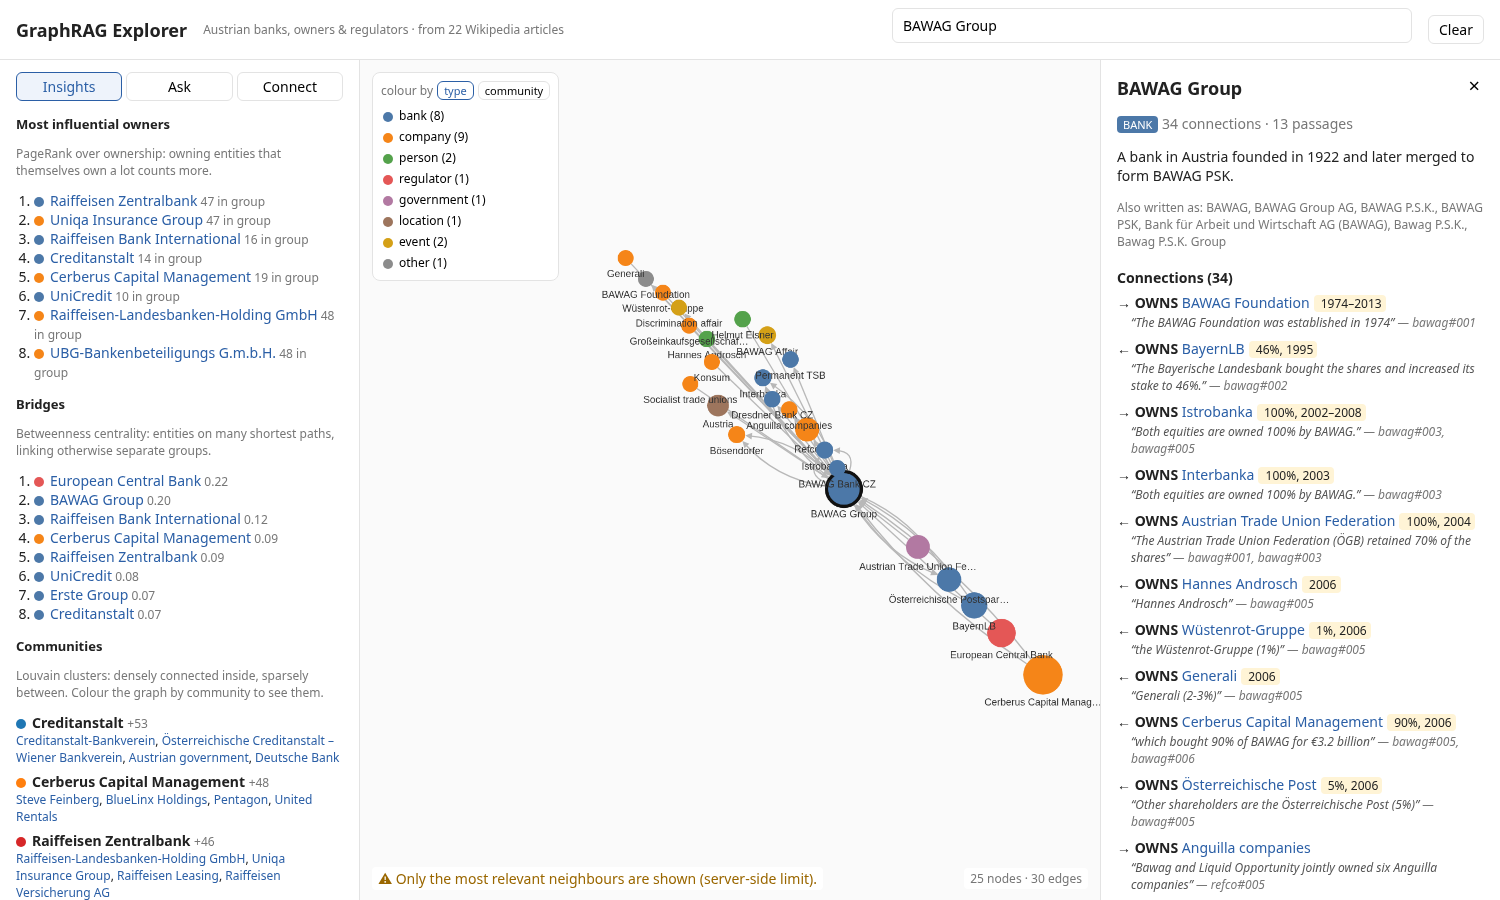
\includegraphics[width=\linewidth]{img/2_bawag.png}
    \end{column}
  \end{columns}
\end{frame}

%-------------------------------------------------------------
\begin{frame}{Extraktion: das LLM schlägt vor, der Code prüft}
  \begin{itemize}
    \item Ein LLM-Call pro Chunk, \hl{Pydantic-Schema} als Structured Output
    \item Feste Typlisten: 8 Entitätstypen, 9 Relationstypen
    \item Eine \hl{kanonische Richtung}: „A ist Tochter von B“ wird zu \texttt{B OWNS A}
    \item Jedes Element wird einzeln validiert: eine fehlerhafte Relation verwirft nicht den ganzen Chunk
    \item \hl{Grounding-Check}: das Belegzitat muss vom Chunk gestützt sein
  \end{itemize}
  \story{Exaktes Substring-Grounding verwarf 73 Relationen, davon \textasciitilde70 korrekte
    (Zitate mit „\ldots“). Mit Wort-Abdeckung bleibt 1 übrig, und es erkennt trotzdem,
    wenn das Modell Umlaute verschluckt („\"Osterreichische“ $\rightarrow$ „sterr ischische“).}
\end{frame}

%-------------------------------------------------------------
\begin{frame}{Entity Resolution: falsche Merges sind schlimmer als Splits}
  \begin{itemize}
    \item Normalisieren: Groß-/Kleinschreibung, Akzente, \texttt{\"o}$\rightarrow$\texttt{oe}, Rechtsformen (AG, GmbH, a.s.)
    \item Danach eine \hl{kuratierte Alias-Datei}: jeder Merge ist explizit und prüfbar
    \item Typ per Mehrheitsentscheid (das LLM sagt einmal BANK, einmal COMPANY)
    \item In einer Bank würde ein Merge zweier „Raiffeisen \ldots“ \hl{Eigentum erfinden}
  \end{itemize}
  \story{Die Kette ÖGB $\rightarrow$ BAWAG $\leftarrow$ Cerberus war unterbrochen: das LLM schrieb
    in einem Chunk „Cerberus“ und „ÖGB“, in anderen die vollen Namen. Außerdem ist
    „Ceberus“ ein Tippfehler in Wikipedia selbst.}
\end{frame}

%-------------------------------------------------------------
\begin{frame}{Retrieval: Graph-Modus}
  \begin{enumerate}
    \item \hl{Hybride Suche}: Vektor + Volltext, fusioniert mit Reciprocal Rank Fusion (Ränge statt Scores)
    \item \hl{Seeds}: Entitäten, deren Namen in der Frage vorkommen
    \item \hl{Pfade} zwischen den Seeds, dann Breitensuche mit Knotenlimit
    \item Orte sind nie Zwischenschritte („beide sitzen in Wien“)
    \item Chunks hinter den Kanten + Reranker; \hl{jede Pfadkante hat einen reservierten Platz} für ihren Beleg
    \item Antwort mit Zitaten; der Code entfernt Zitate von Passagen, die das Modell nicht gesehen hat
  \end{enumerate}
  \story{Ein Hub-Filter nach Knotengrad blockierte die wichtigsten Banken: hier \emph{sind}
    die Knoten mit hohem Grad die Antwort. Der Typ (Ort) war das richtige Signal.}
\end{frame}

%-------------------------------------------------------------
\begin{frame}{Funktionen zum Entdecken}
  \begin{itemize}
    \item \hl{Zeit und Anteil an den Kanten}: ein zweiter, gezielter LLM-Durchlauf (15 Calls, rund 200 Kanten)\\
      \small BayernLB 46\,\% (1995) $\rightarrow$ ÖGB 100\,\% (2004) $\rightarrow$ Cerberus 90\,\% (2006) $\rightarrow$ GoldenTree 21,8\,\%
    \item \hl{Graph-Analytik} bei der Ingestion (networkx):
      \begin{itemize}\small
        \item PageRank über umgekehrte Eigentumskanten: wer kontrolliert am meisten
        \item Betweenness: Brücken zwischen Gruppen (EZB, BAWAG)
        \item Louvain-Communities: Erste + CEE-Banken, UniCredit + Bank Austria, \ldots
      \end{itemize}
    \item Pfadsuche ohne LLM: sofort und kostenlos
  \end{itemize}
  \story{„SIA“ war unter den Top-5-Eigentümern. Aus ``UniCredit verkaufte ihr \emph{Kartengeschäft}
    an SIA'' war \texttt{SIA ACQUIRED UniCredit} geworden. Eine falsche Kante verzerrte eine globale Kennzahl.}
\end{frame}

%-------------------------------------------------------------
\begin{frame}{Engineering für unzuverlässige Free-Tier-APIs}
  \begin{itemize}
    \item Timeouts, Retries mit Backoff, clientseitiger \hl{Rate Limiter}
    \item \hl{Fallback-Kette} von Modellen bei 503 und bei Quota-Fehlern
    \item \hl{Inhaltsadressierter Cache}: erneute Läufe sind kostenlos und reproduzierbar
    \item Alles-oder-nichts-Schreiben: ein fehlgeschlagener Lauf schreibt nichts und setzt aus dem Cache fort
    \item API: Ressourcen über Lifespan, Dependency Injection, Request-IDs, Liveness vs.\ Readiness
  \end{itemize}
  \story{\texttt{gemini-3.5-flash} erlaubt \hl{20 Requests pro Tag}, die Ingestion braucht 160.
    Außerdem zählt der Free Tier jeden Text in einem Embedding-Batch als eigenen Request.}
\end{frame}

%-------------------------------------------------------------
\begin{frame}{Evaluationsdesign}
  \begin{itemize}
    \item 28 Fragen: 13 Multi-Hop, 10 Lookup, 5 korpusweite
    \item Erstellt aus dem \hl{Text, nicht aus dem Graphen}: sonst würde der Graph-Modus an seinen eigenen Daten gemessen
    \item Metriken: Recall@8, Complete@8, LLM-Judge, Entity Recall, Latenz, Tokens
    \item Judge von einem \hl{anderen Anbieter} (Groq) als die Antworten (Gemini): Self-Preference-Bias
    \item \hl{Gepaarte} Statistik: Bootstrap-Konfidenzintervalle, McNemar, Wilcoxon
    \item Reliabilität des Judges: zweiter Judge (Qwen), Cohens $\kappa$
  \end{itemize}
\end{frame}

%-------------------------------------------------------------
\begin{frame}{Runde 1 (ursprünglicher Prompt): kein messbarer Unterschied}
  \centering
  \begin{tabular}{lcc}
    \toprule
    & Vektor & Graph \\
    \midrule
    Judge-Score & 0,91 [0,80; 0,98] & 0,91 [0,84; 0,98] \\
    korrekt & 24/28 & 23/28 \\
    Recall@8 & 0,90 & 0,89 \\
    LLM-Latenz p50 / Tokens & 1,7\,s / 2,8k & 2,5\,s / 3,4k \\
    \bottomrule
  \end{tabular}
  \vspace{8pt}
  \begin{itemize}\small
    \item Differenz +0,00 [$-$0,05; +0,05], McNemar p = 1,0
    \item \hl{Deckeneffekt}: generierte Fragen nennen ihre Entitäten, die Vektorsuche findet beide Passagen
    \item Beide Modi scheitern an \hl{korpusweiten} Fragen: Top-k kann keine Aggregation einsammeln
  \end{itemize}
\end{frame}

%-------------------------------------------------------------
\begin{frame}{Runde 2: ein vorab registrierter, schwerer Test}
  \begin{itemize}\small
    \item Hypothese \hl{vor} dem Lauf festgelegt: der Graph gewinnt bei Verbindungsfragen
    \item 8 Fragen „How is A connected to C?“, die Brücke wird nirgends genannt
    \item Prompt-Fix nur auf diesen neuen Fragen evaluiert: \hl{kein Tuning auf dem Testset}
  \end{itemize}
  \centering\small
  \begin{tabular}{lcc}
    \toprule
    & Vektor & Graph \\
    \midrule
    Judge-Score & 0,38 & 0,44 \\
    korrekt & 3/8 & 2/8 \\
    Recall@8 & 0,56 & 0,50 \\
    Recall@8 \hl{ohne Reranker} & \hl{0,81} & 0,56 \\
    \bottomrule
  \end{tabular}
  \vspace{6pt}
  \begin{itemize}\small
    \item Differenz +0,06 [$-$0,12; +0,25]: \hl{Hypothese nicht bestätigt}
    \item Der Reranker schadet Verbindungsfragen am meisten (Vektor-Recall 0,81 $\rightarrow$ 0,56)
    \item Regressionscheck auf den alten 28: nichts kaputt (Graph 0,93 vs.\ Vektor 0,91)
    \item Zwei Judges stimmen bei 51/56 + 13/16 Antworten überein, Cohens $\kappa$ = 0,62 / 0,69
  \end{itemize}
\end{frame}

%-------------------------------------------------------------
\begin{frame}{Was ich gelernt habe}
  \begin{columns}[T]
    \begin{column}{0.48\textwidth}
      \hl{Wo der Graph hilft}
      \begin{itemize}\small
        \item Exploration: Pfade, Nachbarschaften, Rankings
        \item Erklärbarkeit: jede Kante hat ein Quellzitat
        \item Struktur: Zeit und Anteil bei Eigentum
        \item Fehler werden sichtbar (SIA, Cerberus)
      \end{itemize}
    \end{column}
    \begin{column}{0.48\textwidth}
      \hl{Wo (noch) nicht}
      \begin{itemize}\small
        \item QA-Genauigkeit auf einem kleinen, sauberen Korpus
        \item Fehlende Extraktionen begrenzen ihn: „Addiko wurde aus der Hypo abgespalten“ wurde nie zur Kante
        \item Globale Fragen brauchen Graph-Abfragen, nicht Top-k
      \end{itemize}
    \end{column}
  \end{columns}
  \vspace{10pt}
  \centering\small
  Ein ehrlich gemessenes negatives Ergebnis ist auch ein Ergebnis.
\end{frame}

%-------------------------------------------------------------
\begin{frame}{Nächste Schritte}
  \begin{itemize}
    \item Reranker im Graph-Modus weglassen oder ersetzen (er ist auf Web-Suchanfragen trainiert)
    \item Aggregationsmodus für korpusweite Fragen (Graph-Abfrage statt Top-k)
    \item Höherer Recall bei der Extraktion: zweiter Durchlauf für Chunks mit wenigen Relationen
    \item Zeitleisten-Filter im Explorer (die Daten sind schon da)
    \item In einer Bank: selbst gehostete oder in der EU gehostete Modelle, Snowflake als Dokumentquelle,
          Airflow für geplante Re-Ingestion
  \end{itemize}
\end{frame}

%-------------------------------------------------------------
\begin{frame}
  \centering
  \Large Danke. Fragen?
  \vspace{12pt}

  \small Code, Evaluation und Notizen: Repository \texttt{graphRAG-demo}
\end{frame}

%-------------------------------------------------------------
\appendix
\begin{frame}{Backup: Ask mit hervorgehobenem Pfad}
  \centering
  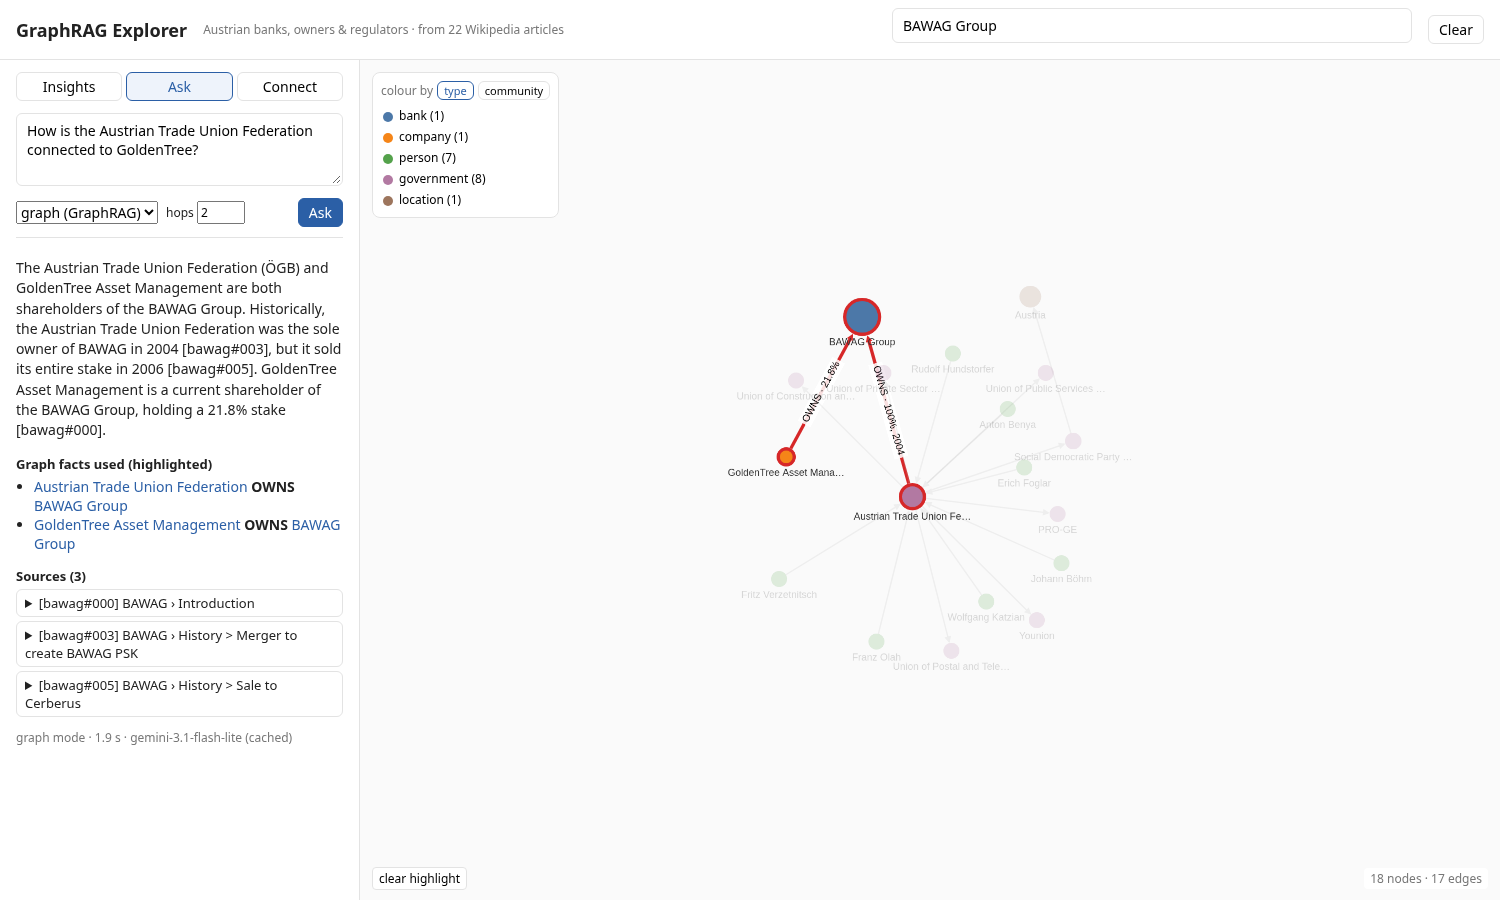
\includegraphics[width=0.85\linewidth]{img/4_ask.png}
\end{frame}

\begin{frame}{Backup: Pfadsuche}
  \centering
  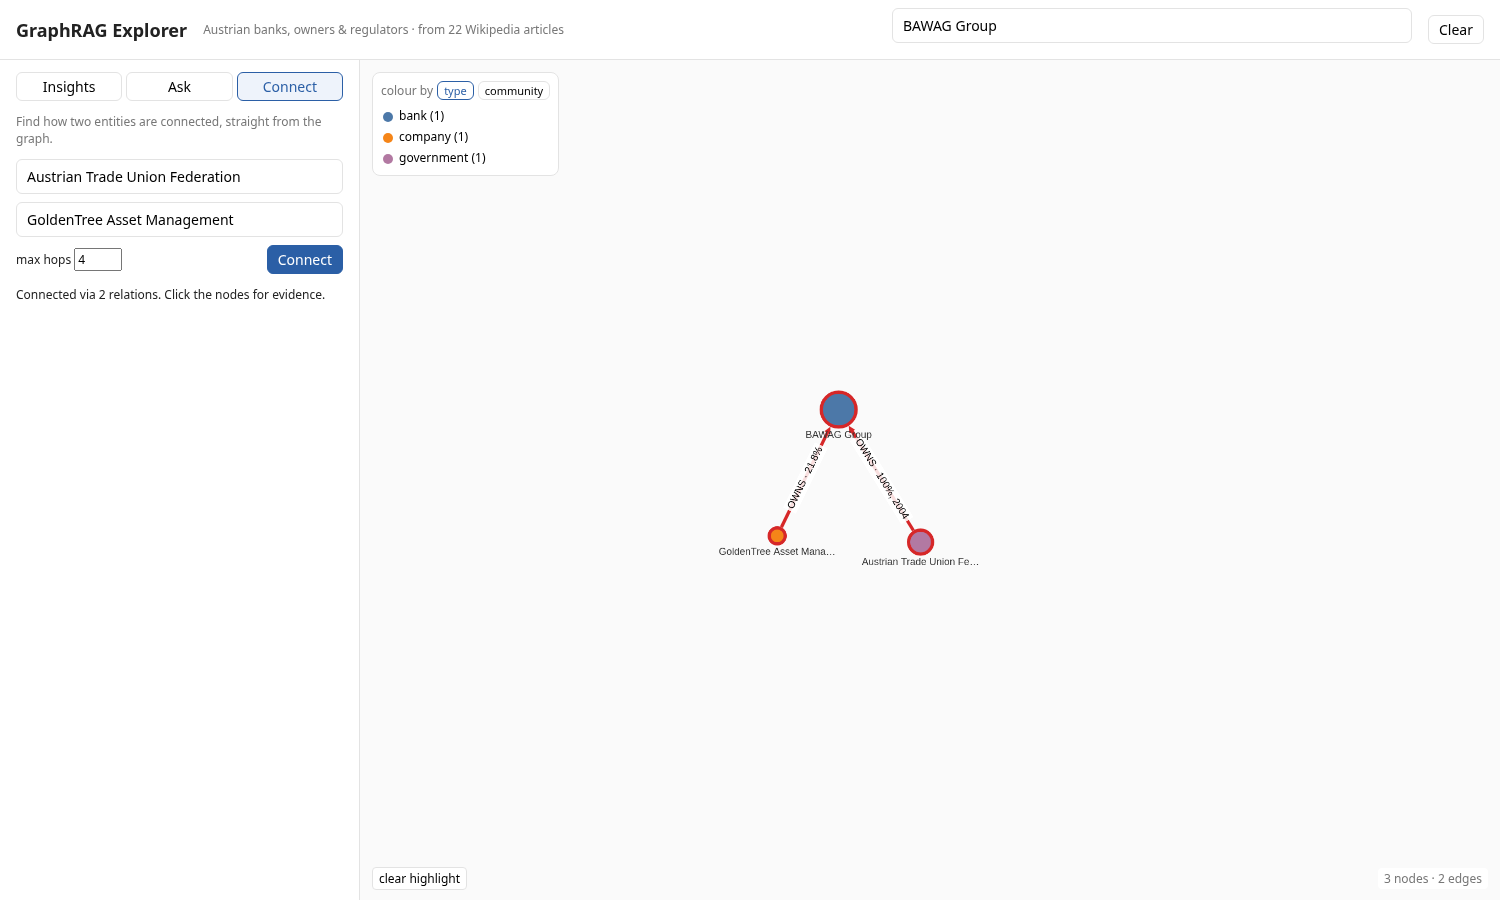
\includegraphics[width=0.85\linewidth]{img/3_path.png}
\end{frame}

\end{document}
